\documentclass[xcolor=pdflatex,dvipsnames,table]{beamer}
\usepackage{epsfig,graphicx}
\usepackage{palatino}
\usepackage{fancybox}
\usepackage{relsize}
\usepackage[procnames]{listings}
\usepackage{hyperref}
\usepackage{qtree} % needed?
\usepackage{booktabs}
\usepackage{dirtree}
\usepackage[normalem]{ulem}


% fatter TT font
\renewcommand*\ttdefault{txtt}
% another TT, suggested by Alex
% \usepackage{inconsolata}
% \usepackage[T1]{fontenc} % needed as well?


\newcommand{\scale}{0.7}

\newcommand{\todo}[1]{{\emph{TODO: #1}}}
\newcommand{\martin}[1]{{\color{blue} Martin: #1}}
\newcommand{\abcdef}[1]{{\color{red} Author2: #1}}

% uncomment following for final submission
%\renewcommand{\todo}[1]{}
%\renewcommand{\martin}[1]{}
%\renewcommand{\author2}[1]{}

\newcommand{\code}[1]{{\texttt{#1}}}

\hypersetup{
  linkcolor  = black,
%  citecolor  = blue,
  urlcolor   = blue,
  colorlinks = true,
}

\beamertemplatenavigationsymbolsempty
\setbeamertemplate{footline}[frame number]





\newif\ifbook
% shared in slides and book

\lstdefinelanguage{chisel}{
  morekeywords={abstract,case,catch,class,def,%
    do,else,extends,false,final,finally,%
    for,if,implicit,import,match,mixin,%
    new,null,object,override,package,%
    private,protected,requires,return,sealed,%
    super,this,throw,trait,true,try,%
    type,val,var,while,with,yield},
  otherkeywords={=>,<-,<\%,<:,>:,\#,@},
  sensitive=true,
  morecomment=[l]{//},
  morecomment=[n]{/*}{*/},
  morestring=[b]",
  morestring=[b]',
  morestring=[b]"""
}

\usepackage{color}
\definecolor{dkgreen}{rgb}{0,0.6,0}
\definecolor{gray}{rgb}{0.5,0.5,0.5}
\definecolor{mauve}{rgb}{0.58,0,0.82}

% Default settings for code listings
\ifbook
\lstset{%frame=lines,
  language=chisel,
  aboveskip=3mm,
  belowskip=3mm,
  showstringspaces=false,
  columns=fixed, % basewidth=\mybasewidth,
  basicstyle={\small\ttfamily},
  numbers=none,
  numberstyle=\footnotesize,
  % identifierstyle=\color{red},
  breaklines=true,
  breakatwhitespace=true,
  procnamekeys={def, val, var, class, trait, object, extends},
  % procnamestyle=\ttfamily,
  tabsize=2,
  float
}
\else
\lstset{%frame=lines,
  language=chisel,
  aboveskip=3mm,
  belowskip=3mm,
  showstringspaces=false,
  columns=fixed, % basewidth=\mybasewidth,
  basicstyle={\small\ttfamily},
  numbers=none,
  numberstyle=\footnotesize\color{gray},
  % identifierstyle=\color{red},
  keywordstyle=\color{blue},
  commentstyle=\color{dkgreen},
  stringstyle=\color{mauve},
  breaklines=true,
  breakatwhitespace=true,
  procnamekeys={def, val, var, class, trait, object, extends},
  procnamestyle=\ttfamily\color{red},
  tabsize=2,
  float
}
\fi

\lstnewenvironment{chisel}[1][]
{\lstset{language=chisel,#1}}
{}

\newcommand{\shortlist}[1]{{\lstinputlisting[nolol]{#1}}}

\newcommand{\longlist}[3]{{\lstinputlisting[float, caption={#2}, label={#3}, frame=tb, captionpos=b]{#1}}}

\newcommand{\verylonglist}[3]{{\lstinputlisting[caption={#2}, label={#3}, frame=tb, captionpos=b]{#1}}}


\title{Finite State Machine with Datapath}
\author{Martin Schoeberl}
\date{\today}
\institute{Technical University of Denmark\\
Embedded Systems Engineering}

\begin{document}

\begin{frame}
\titlepage
\end{frame}

\begin{frame}[fragile]{Overview}
\begin{itemize}
\item Counter based circuits
\item Finite-state machines (FSMs) 
\item FSM with Datapath
\end{itemize}
\end{frame}



\begin{frame}[fragile]{Last Lab}
\begin{itemize}
\item Generate a timing and a free running counter
\begin{itemize}
\item Two counters
\item One for the counting from 0 to 15
\item One to generate a \emph{tick} at about 2 Hz
\end{itemize}
\item Did you finish the exercises?
\item I will show the solution later
\end{itemize}
\end{frame}

\begin{frame}[fragile]{Generating Timing with Counters}
\begin{itemize}
\item Generate a \code{tick} at a lower frequency
\item We used it in Lab 1 for the blinking LED
\item Used for last lab
\item Use it for driving the display multiplexing at 1~kHz
\end{itemize}
\begin{figure}
  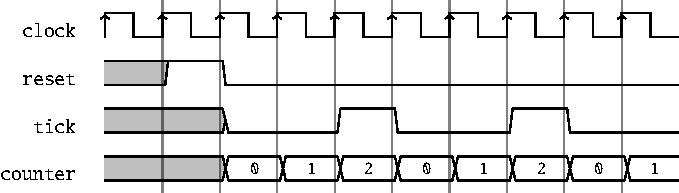
\includegraphics[scale=0.8]{../figures/tick_wave}
\end{figure}
\end{frame}


\begin{frame}[fragile]{The Tick Generation}
\shortlist{../code/sequ_tick_gen.txt}
\end{frame}

\begin{frame}[fragile]{Using the Tick}
\begin{itemize}
\item A counter running at a \emph{slower frequency}
\item By using the \code{tick} as an enable signal
\end{itemize}
\shortlist{../code/sequ_tick_counter.txt}
\end{frame}

\begin{frame}[fragile]{The \emph{Slow} Counter}
\begin{itemize}
\item Incremented every \code{tick}
\end{itemize}
\begin{figure}
  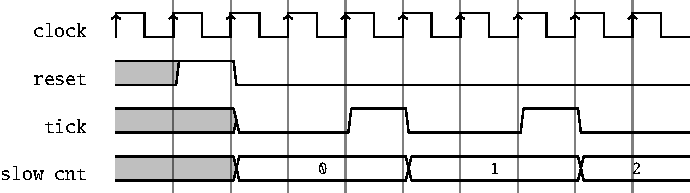
\includegraphics[scale=0.8]{../figures/tick_count_wave}
\end{figure}
\end{frame}

\begin{frame}[fragile]{What is the Use of This \emph{Slow} Counter?}
\begin{itemize}
\item This was your lab exercise last week!
\item Is a preparation for the display multiplexing (next week)
\item Then you need to generate a timing of 1 kHz (1 ms)
\end{itemize}
\end{frame}

\begin{frame}[fragile]{One Possible Solution for Last Lab}
\begin{chisel}
  val MAX_CNT = 50000000.U // use a small value for waveform viewing
  
  val tickCntReg = RegInit(0.U(32.W))
  val cntReg = RegInit(0.U(4.W))
  
  val tick = tickCntReg === MAX_CNT
  tickCntReg := Mux(tick, 0.U, tickCntReg + 1.U)
  when (tick) {
    cntReg := cntReg + 1.U
  }
  
  val m = Module(new SevenSegDec())
  m.io.in := cntReg
  sevSeg := m.io.out
\end{chisel}
\end{frame}

\begin{frame}[fragile]{A Self-Running Tester}
\begin{itemize}
\item \code{CountSevenSeg} is a self-running circuit
\item Has no input
\item Needs no stimuli (\code{poke})
\item Just run for a few cycles
\end{itemize}
\begin{chisel}
class SevenSegTest(dut: CountSevenSeg) extends PeekPokeTester(dut) {
  step(100)
}
\end{chisel}
\end{frame}

\begin{frame}[fragile]{Call the Tester}
\begin{itemize}
\item Using here ScalaTest
\item Note \code{Driver.execute}
\item Note \code{Array("--generate-vcd-output", "on")}
\end{itemize}
\begin{chisel}
class SevenSegCountSpec extends
  FlatSpec with Matchers {
  
  "SevenSegTest " should "pass" in {
      chisel3.iotesters.Driver.execute(
      Array("--generate-vcd-output", "on"),
      () => new CountSevenSeg)
        { c => new SevenSegTest(c)}
        should be (true)
	}
}
\end{chisel}
\end{frame}

\begin{frame}[fragile]{Running the Test}
\begin{itemize}
\item Does not really do any testing
\item Just generated the waveform for debugging
\item Just running 100 cycles does not show much
\item Increase the number of running cycles to 100000000?
\item Or use a different constant for testing?
\item Let us explore now
\item This issue will be the same for your display multiplexing
\end{itemize}
\end{frame}


\begin{frame}[fragile]{A Timer}
\begin{itemize}
\item Like a kitchen timer
\item Start by loading a timeout value
\item Count down till 0
\item Assert \code{done} when finished
\end{itemize}
\end{frame}

\begin{frame}[fragile]{One-Shot Timer}
\begin{figure}
  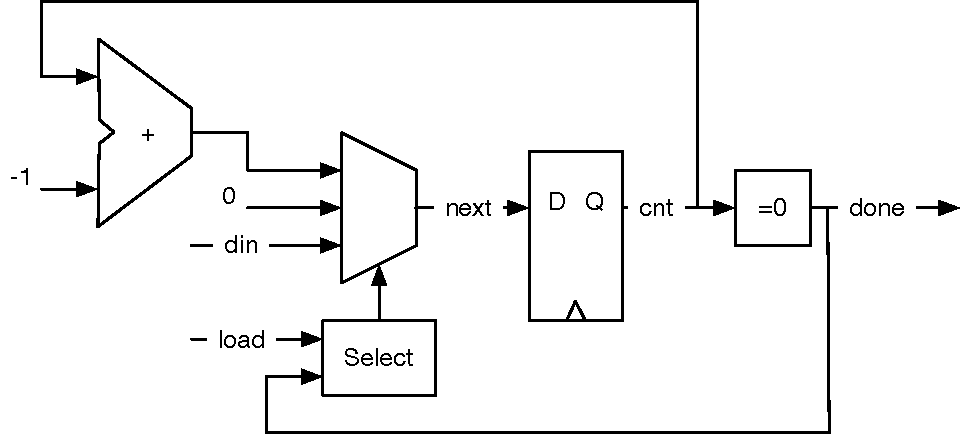
\includegraphics[scale=\scale]{../figures/timer}
\end{figure}
\end{frame}

\begin{frame}[fragile]{One-Shot Timer}
\shortlist{../code/timer.txt}
\end{frame}

\begin{frame}[fragile]{A 4 Stage Shift Register}
\begin{figure}
  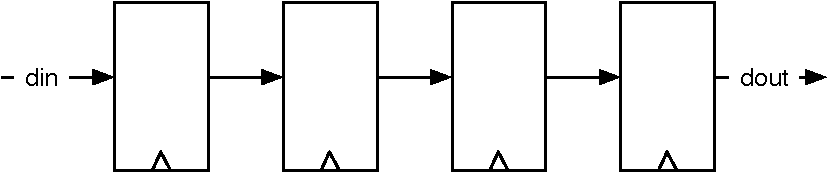
\includegraphics[scale=\scale]{../figures/shiftregister}
\end{figure}
\shortlist{../code/shift_register.txt}
\end{frame}


\begin{frame}[fragile]{A Shift Register with Parallel Output}
\begin{figure}
  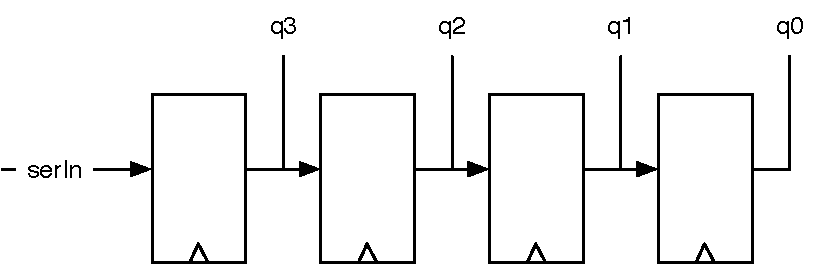
\includegraphics[scale=\scale]{../figures/shiftreg-paraout}
\end{figure}
\shortlist{../code/shift_paraout.txt}
\end{frame}

\begin{frame}[fragile]{A Shift Register with Parallel Load}
\begin{figure}
  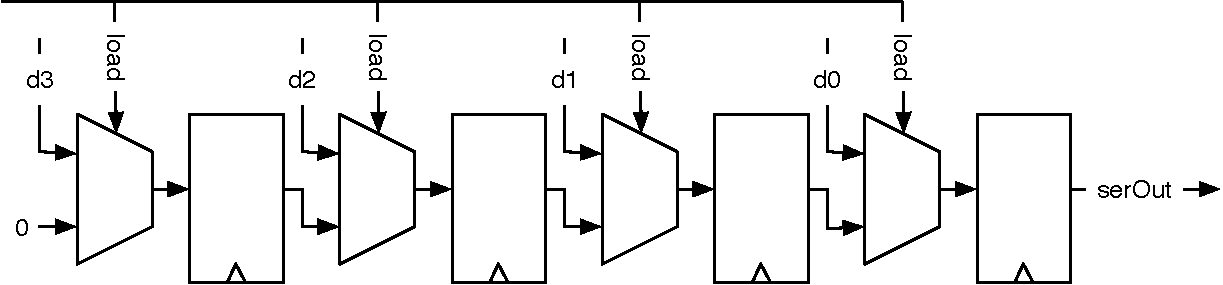
\includegraphics[scale=0.5]{../figures/shiftreg-paraload}
\end{figure}
\shortlist{../code/shift_paraload.txt}
\end{frame}


\begin{frame}[fragile]{A Simple Circuit}
\begin{itemize}
\item What does the following circuit?
\item Is this related to a finite-state machine?
\end{itemize}
\begin{figure}
  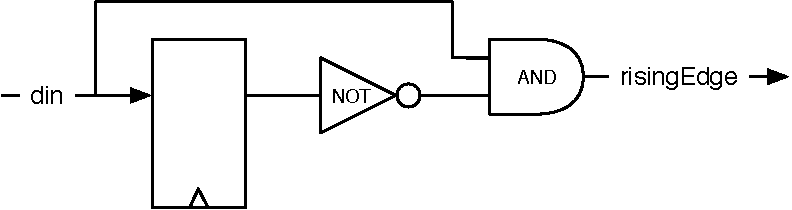
\includegraphics[scale=\scale]{../figures/fsm-rising}
\end{figure}
\end{frame}

\begin{frame}[fragile]{Finite-State Machine (FSM)}
\begin{itemize}
\item Has a register that contains the state
\item Has a function to computer the next state
\begin{itemize}
\item Depending on current state and input
\end{itemize}
\item Has an output depending on the state
\begin{itemize}
\item And maybe on the input as well
\end{itemize}
\item Every synchronous circuit can be considered a finite state machine
\item However, sometimes the state space is a little bit too large
\end{itemize}
\end{frame}

\begin{frame}[fragile]{Basic Finite-State Machine}
\begin{itemize}
\item A state register
\item Two combinational blocks
\end{itemize}
\begin{figure}
  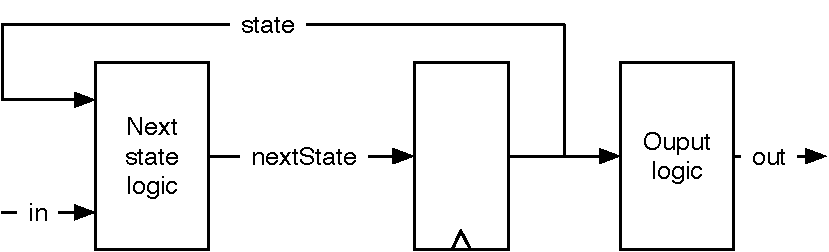
\includegraphics[scale=\scale]{../figures/fsm}
\end{figure}
\end{frame}

\begin{frame}[fragile]{State Diagram}
\begin{figure}
  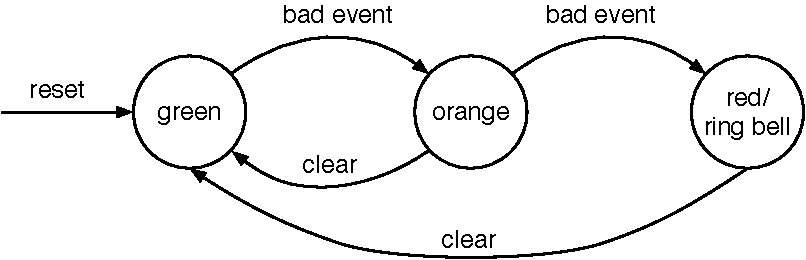
\includegraphics[scale=\scale]{../figures/state-diag-moore}
\end{figure}
\begin{itemize}
\item States and transitions depending on input values
\item Example is a simple alarm FSM
\item Nice visualization
\item Will not work for large FSMs
\item Complete code in the Chisel book
\end{itemize}
\end{frame}


\begin{frame}[fragile]{State Table for the Alarm FSM}
\begin{table}
\centering
\begin{tabular}{ccccc}
\toprule
& \multicolumn{2}{c}{Input} \\
\cmidrule{2-3}
State &  Bad event & Clear & Next state & Ring bell \\
\midrule
green & 0 & 0 & green & 0 \\
green & 1 & - & orange & 0 \\
orange & 0 & 0 & orange & 0 \\
orange & 1 & - & red & 0 \\
orange & 0 & 1 & green & 0 \\
red & 0 & 0 & red & 1 \\
red & 0 & 1 & green & 1 \\
\bottomrule
\end{tabular}
\label{tab:state:table}
\end{table}
\end{frame}

\begin{frame}[fragile]{The Input and Output of the Alarm FSM}
\begin{itemize}
\item Two inputs and one output
\end{itemize}
\shortlist{../code/simple_fsm_io.txt}
\end{frame}

\begin{frame}[fragile]{Encoding the State}
\begin{itemize}
\item We can optimize state encoding
\item Two common encodings are: binary and one-hot
\item We leave it to the synthesize tool
\item Use symbolic names with an \code{Enum}
\item Note the number of states in the \code{Enum} construct
\item We use a Scala list with the \code{::} operator
\end{itemize}
\shortlist{../code/simple_fsm_states.txt}
\end{frame}

\begin{frame}[fragile]{Start the FSM}
\begin{itemize}
\item We have a starting state on reset
\end{itemize}
\shortlist{../code/simple_fsm_register.txt}
\end{frame}


\begin{frame}[fragile]{The Next State Logic}
\shortlist{../code/simple_fsm_next.txt}
\end{frame}

\begin{frame}[fragile]{The Output Logic}
\shortlist{../code/simple_fsm_output.txt}
\end{frame}

\begin{frame}[fragile]{Summary on the Alarm Example}
\begin{itemize}
\item Three elements:
\begin{enumerate}
\item State register
\item Next state logic
\item Output logic
\end{enumerate}
\item This was a so-called Moore FSM
\item There is also a FSM type called Mealy machine
\end{itemize}
\end{frame}

\begin{frame}[fragile]{A so-called Mealy FSM}
\begin{itemize}
\item Similar to the former FSM
\item Output also depends in the input
\item It is \emph{faster}
\item Less composable (draw it)
\end{itemize}
\begin{figure}
  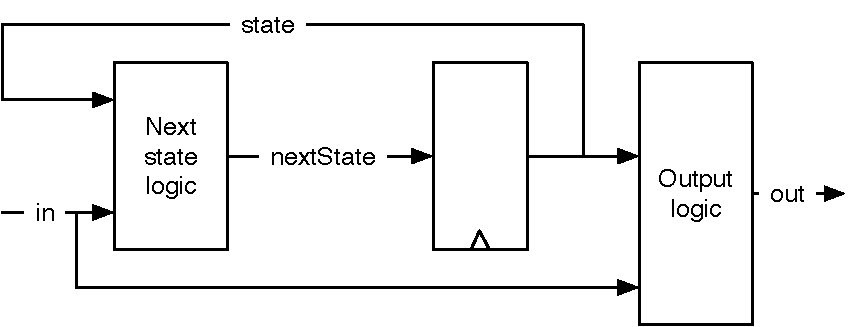
\includegraphics[scale=\scale]{../figures/mealy}
\end{figure}
\end{frame}

\begin{frame}[fragile]{The Mealy FSM for the Rising Edge}
\begin{itemize}
\item That was our starting example
\item Output is also part of the transition arrows
\end{itemize}
\begin{figure}
  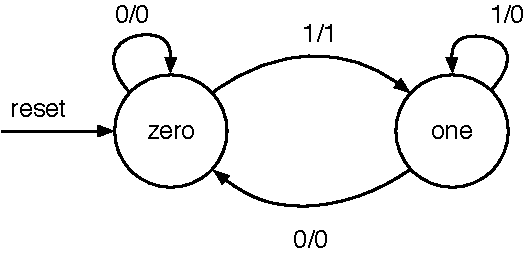
\includegraphics[scale=\scale]{../figures/state-diag-mealy}
\end{figure}
\end{frame}

\begin{frame}[fragile]{The Mealy Solution}
\begin{itemize}
\item Show code from the book as it is too long for slides
\end{itemize}
\end{frame}

\begin{frame}[fragile]{State Diagram for the Moore Rising Edge Detection}
\begin{itemize}
\item We need three states
\item Show the code
\end{itemize}
\begin{figure}
  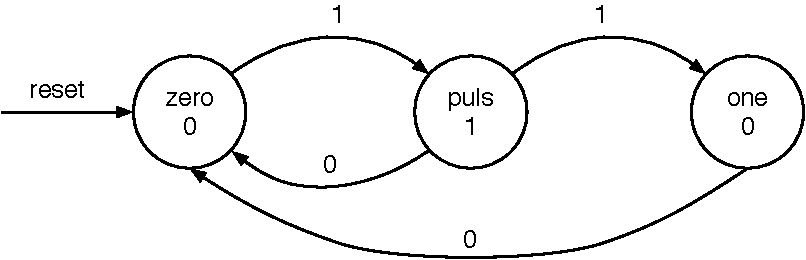
\includegraphics[scale=\scale]{../figures/state-diag-rising-moore}
\end{figure}
\end{frame}

\begin{frame}[fragile]{Comparing with a Timing Diagram}
\begin{itemize}
\item Moore is delayed one clock cycle compared to Mealy
\end{itemize}
\begin{figure}
  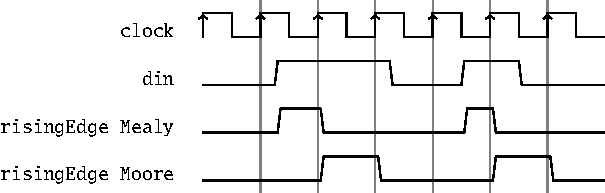
\includegraphics[scale=1]{../figures/rising}
\end{figure}
\end{frame}

\begin{frame}[fragile]{What is Better?}
\begin{itemize}
\item It depends ;-)
\item Moore is on the save side
\item Moore is composable
\item Mealy has \emph{faster} reaction
\item Both are tools in you toolbox
\item Keep it simple with your vending machine and use a Moore FSM
\end{itemize}
\end{frame}

\begin{frame}[fragile]{Another Simple FSM}
\begin{itemize}
\item a FSM for a single word buffer
\item Just two symbols for the state machine
\end{itemize}
\begin{chisel}
  val empty :: full :: Nil = Enum(2)
\end{chisel}
\end{frame}

\begin{frame}[fragile]{Finite State Machine for a Buffer}
\begin{chisel}
  val empty :: full :: Nil = Enum(2)
  val stateReg = RegInit(empty)
  val dataReg = RegInit(0.U(size.W))

  when(stateReg === empty) {
    when(io.enq.write) {
      stateReg := full
      dataReg := io.enq.din
    }
  }.elsewhen(stateReg === full) {
    when(io.deq.read) {
      stateReg := empty
    }
  }
\end{chisel}
\begin{itemize}
\item A simple buffer for a bubble FIFO
\end{itemize}
\end{frame}


\begin{frame}[fragile]{FSM with Datapath}
\begin{itemize}
\item A type of computing machine
\item Consists of a finite-state machine (FSM) and a datapath
\item The FSM is the master (the controller) of the datapath
\item The datapath has computing elements
\begin{itemize}
\item E.g., adder, incrementer, constants, multiplexers, ...
\end{itemize}
\item The datapath has storage elements (registers)
\begin{itemize}
\item E.g., sum of money payed, count of something, ...
\end{itemize}
\end{itemize}
\end{frame}

\begin{frame}[fragile]{FSM-Datapath Interaction}
\begin{itemize}
\item The FSM controls the datapath
\begin{itemize}
\item For example, add 2 to the sum
\end{itemize}
\item By controlling multiplexers
\begin{itemize}
\item For example, select how much to add
\item Not adding means selecting 0 to add
\end{itemize}
\item Which value goes where
\item The FSM logic also depends on datapath output
\begin{itemize}
\item Is there enough money payed to release a can of soda?
\end{itemize}
\item FSM and datapath interact
\end{itemize}
\end{frame}


\begin{frame}[fragile]{Popcount Example}
\begin{itemize}
\item An FSMD that computes the popcount
\item Also called the Hamming weight
\item Compute the number of `1's in a word
\item Input is the data word
\item Output is the count
\item Code available at \href{https://github.com/schoeberl/chisel-book/blob/master/src/main/scala/PopCount.scala}{PopCount.scala}
\end{itemize}
\end{frame}

\begin{frame}[fragile]{Popcount Block Diagram}

\begin{figure}
  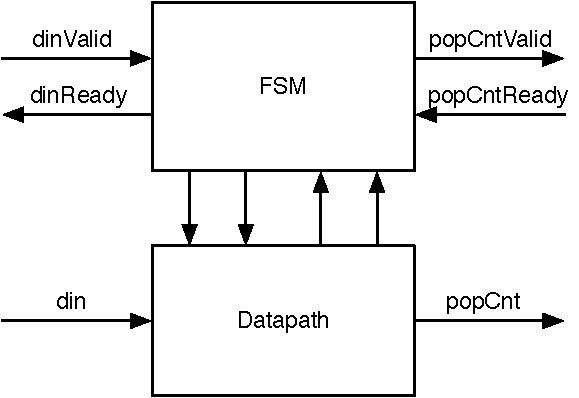
\includegraphics[scale=\scale]{../figures/popcnt-fsmd}
\end{figure}
\end{frame}


\begin{frame}[fragile]{Popcount Connection}
\begin{columns}
\column{0.6\textwidth}
\begin{itemize}
\item Input \code{din} and output \code{popCount}
\item Both connected to the datapath
\item We need some handshaking
\item For data input and for count output
\end{itemize}
\column{0.4\textwidth}
\begin{figure}
  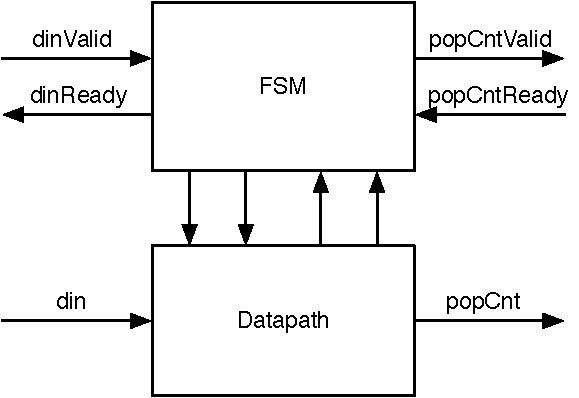
\includegraphics[scale=0.45]{../figures/popcnt-fsmd}
\end{figure}
\end{columns}
\end{frame}

\begin{frame}[fragile]{Popcount Handshake}
\begin{columns}
\column{0.6\textwidth}
\begin{itemize}
\item We use a ready-valid handshake
\item When data is available valid is asserted
\item When the receiver can accept data ready is asserted
\item Transfer takes place when both are asserted
\end{itemize}
\column{0.4\textwidth}
\begin{figure}
  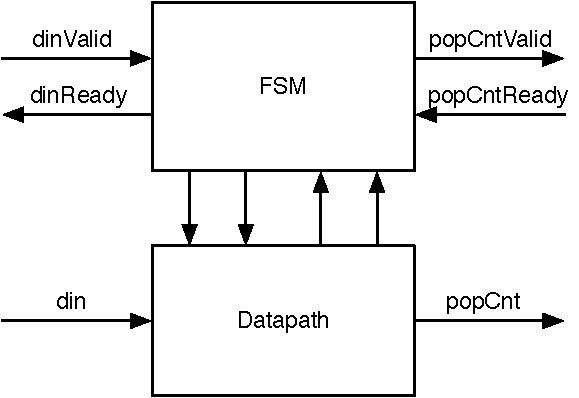
\includegraphics[scale=0.45]{../figures/popcnt-fsmd}
\end{figure}
\end{columns}
\end{frame}


\begin{frame}[fragile]{The FSM}
\begin{figure}
  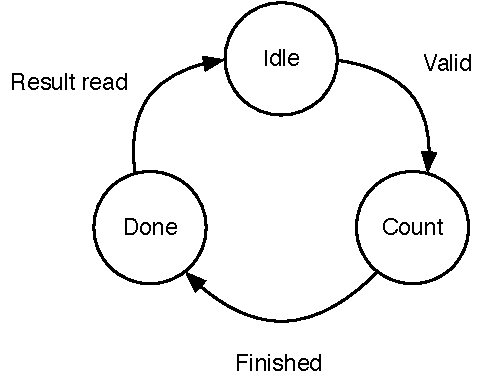
\includegraphics[scale=\scale]{../figures/popcnt-states}
\end{figure}
\begin{itemize}
\item A Very Simple FSM
\item Two transitions depend on input/output handshake
\item One transition on the datapath output
\end{itemize}
\end{frame}

\begin{frame}[fragile]{The Datapath}
\begin{figure}
  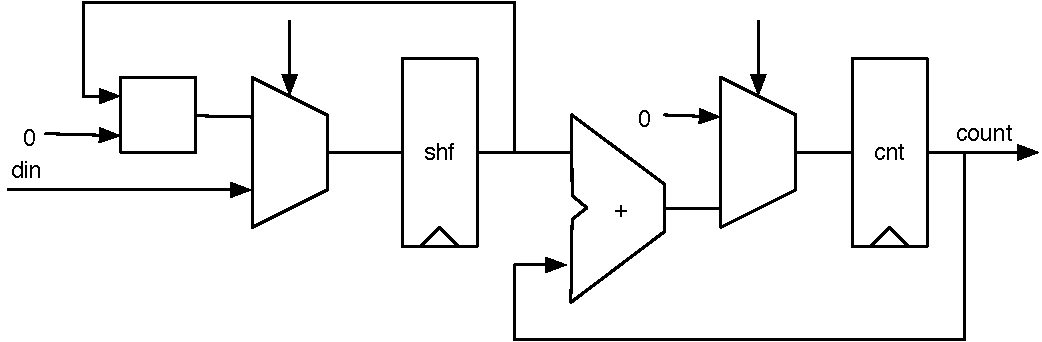
\includegraphics[scale=0.65]{../figures/popcnt-data}
\end{figure}
\end{frame}

\begin{frame}[fragile]{Let's Explore the Code}
\begin{itemize}
\item In \href{https://github.com/schoeberl/chisel-book/blob/master/src/main/scala/PopCount.scala}{PopCount.scala}
\end{itemize}
\end{frame}

\begin{frame}[fragile]{Usage of an FSMD}
\begin{itemize}
\item Maybe the main part your vending machine is an FSMD?
\end{itemize}
\end{frame}




\begin{frame}[fragile]{Today Lab}
\begin{itemize}
\item Paper \& pencil exercises
\item Exercises on FSM
\item From the, now free, Dally book
\item Just sketch the Chisel code
\item On paper or in a plain text editor
\item As usual, show and discuss with a TA
\end{itemize}
\end{frame}

\begin{frame}[fragile]{Summary}
\begin{itemize}
\item We ave interesting teaching constraints
\item We will still be able to build a vending machine
\item Counters make interesting circuits
\item Counter are used to generate timing
\item An FSM can control a datapath
\end{itemize}
\end{frame}


\end{document}

%\begin{frame}[fragile]{xxx}
%\begin{itemize}
%\item yyy
%\end{itemize}
%\end{frame}
